\documentclass{ctexart}
\usepackage[usenames,dvipsnames]{pstricks}
\usepackage{epsfig}
\usepackage{pst-grad} % For gradients
\usepackage{pst-plot} % For axes
\usepackage[space]{grffile} % For spaces in paths
\usepackage{etoolbox} % For spaces in paths
\usepackage{tikz}
\usetikzlibrary{automata, arrows}
\usepackage{color}
\usepackage{subcaption}
\usepackage{float}

\usepackage{geometry}
\geometry{
  a4paper,
  total={170mm,257mm},
  left=20mm,
  top=20mm
}

\title{Compiler Principle Homework}
\author{陈 铮 \\ 软件 42 \\ 学号 2141601026}
\date{April 2017}

\begin{document}

\maketitle

\begin{enumerate}
	\item[3.7] 构造下列正规式相应的DFA
	
	1(0|1)*101
		
	1(1010*|1(010)*1)*0
	
	0*10*10*10*
		
	(00|11)*((01|10)(00|11)*(01|10)(00|11)*)*
	
	\textbf{答:}
    
    \begin{itemize}
        \item 1(0|1)*101
        
        首先根据正规式构造 NFA 如图 \ref{fig:1_1_1}:
        \begin{figure}[H]
            \centering
            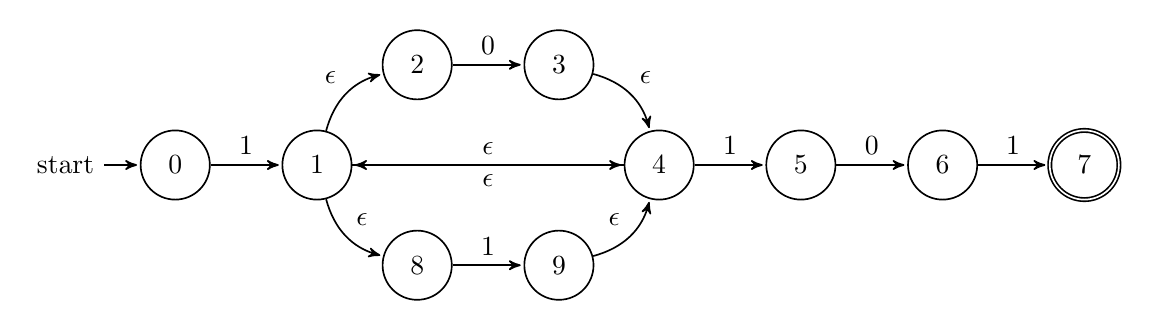
\begin{tikzpicture}[->,>=stealth',shorten >=1pt,auto,node distance=1.8cm,semithick]
            
                \node[initial, state] (0) {0};
                \node[state] (1) [right of=0] {1};
                \node[state] (2) [above right of=1] {2};
                \node[state] (3) [right of=2] {3};
                \node[state] (4) [below right of=3] {4};
                \node[state] (5) [right of=4] {5};
                \node[state] (6) [right of=5] {6};
                \node[accepting, state] (7) [right of=6] {7};
                \node[state] (8) [below right of=1] {8};
                \node[state] (9) [right of=8] {9};
                
                \path 
                (0) edge node {1} (1)
                (1) edge [bend left] node {$\epsilon$} (2)
                    edge node [below] {$\epsilon$} (4)
                    edge [bend right] node {$\epsilon$} (8)
                (2) edge node {0} (3)
                (3) edge [bend left] node {$\epsilon$} (4)
                (4) edge node [above] {$\epsilon$} (1)
                    edge node {1} (5)
                (5) edge node {0} (6)
                (6) edge node {1} (7)
                (8) edge node {1} (9)
                (9) edge [bend right] node {$\epsilon$} (4)
                ;
            \end{tikzpicture}
            \caption{正规式 1(0|1)*101 的完整 NFA}
            \label{fig:1_1_1}
        \end{figure}
        
        边的重定向:消除 $\epsilon$ 边的\textbf{预处理}:
        
        \begin{enumerate}
            \item 状态 1, 4 间存在\textbf{双向 $\epsilon$ 边},说明两个状态完全等价,合并。
            
            将所有指向 4 的边重定向到 1;将所有从 4 发出的边改为从 1 发出。
            
            化简 NFA \ref{fig:1_1_1} 得到 NFA \ref{fig:1_1_2}。
            
            \begin{figure}[H]
                \centering
                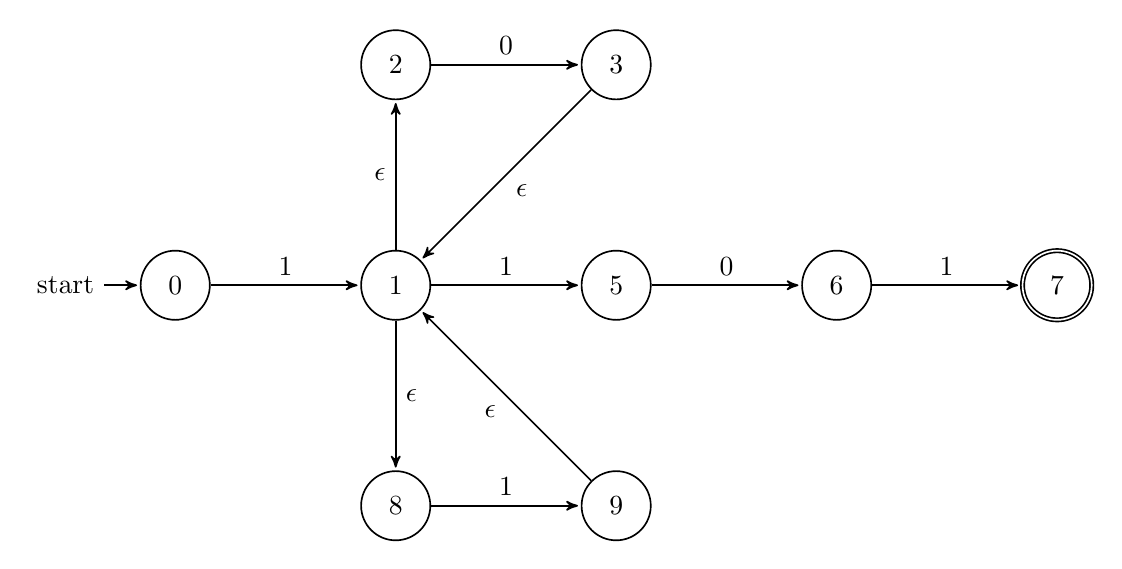
\begin{tikzpicture}[->,>=stealth',shorten >=1pt,auto,node distance=2.8cm,semithick]
                    \node[initial, state] (0) {0};
                    \node[state] (1) [right of=0] {1};
                    \node[state] (2) [above of=1] {2};
                    \node[state] (3) [right of=2] {3};
                    \node[state] (5) [right of=1] {5};
                    \node[state] (6) [right of=5] {6};
                    \node[accepting, state] (7) [right of=6] {7};
                    \node[state] (8) [below of=1] {8};
                    \node[state] (9) [right of=8] {9};
                    
                    \path 
                    (0) edge node {1} (1)
                    (1) edge node {$\epsilon$} (2)
                        edge node {1} (5)
                        edge node {$\epsilon$} (8)
                    (2) edge node {0} (3)
                    (3) edge node {$\epsilon$} (1)
                    (5) edge node {0} (6)
                    (6) edge node {1} (7)
                    (8) edge node {1} (9)
                    (9) edge node {$\epsilon$} (1)
                    ;
                \end{tikzpicture}
                \caption{正规式 1(0|1)*101 的第一次化简 NFA}
                \label{fig:1_1_2}
            \end{figure}
            
            \item 状态 2, 8 仅有 $\epsilon$ 输入;状态 3, 9 仅有 $\epsilon$ 输出。
            
            可重定向边以消除这些状态得到 NFA \ref{fig:1_1_3}:
            
            \begin{figure}[H]
                \centering
                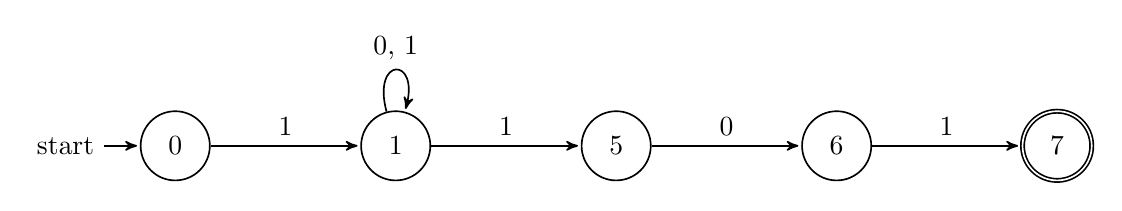
\begin{tikzpicture}[->,>=stealth',shorten >=1pt,auto,node distance=2.8cm,semithick]
                    \node[initial, state] (0) {0};
                    \node[state] (1) [right of=0] {1};
                    \node[state] (2) [right of=1] {5};
                    \node[state] (3) [right of=2] {6};
                    \node[accepting, state] (4) [right of=3] {7};
                    
                    \path 
                    (0) edge node {1} (1)
                    (1) edge [loop above] node {0, 1} (1)
                        edge node {1} (2)
                    (2) edge node {0} (3)
                    (3) edge node {1} (4)
                    ;
                \end{tikzpicture}
                \caption{正规式 1(0|1)*101 的第二次化简 NFA}
                \label{fig:1_1_3}
            \end{figure}

            
        \end{enumerate}
        
        重新标号 NFA \ref{fig:1_1_3} 得到 NFA \ref{fig:1_1_4}:
        
        \begin{figure}[H]
            \centering
            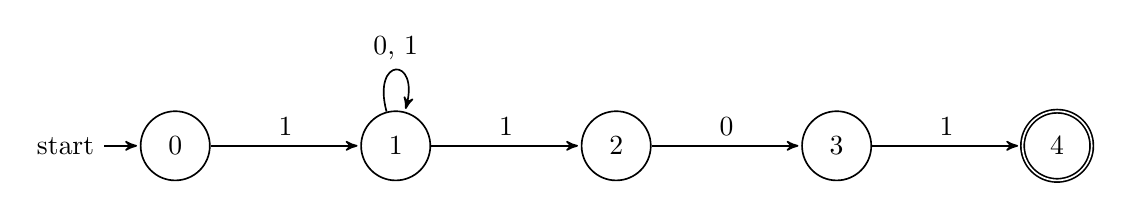
\begin{tikzpicture}[->,>=stealth',shorten >=1pt,auto,node distance=2.8cm,semithick]
            
                \node[initial, state] (0) {0};
                \node[state] (1) [right of=0] {1};
                \node[state] (2) [right of=1] {2};
                \node[state] (3) [right of=2] {3};
                \node[accepting, state] (4) [right of=3] {4};
                
                \path 
                (0) edge node {1} (1)
                (1) edge [loop above] node {0, 1} (1)
                    edge node {1} (2)
                (2) edge node {0} (3)
                (3) edge node {1} (4)
                ;
            \end{tikzpicture}
            \caption{正规式 1(0|1)*101 化简后重新标号的 NFA}
            \label{fig:1_1_4}
        \end{figure}
        
        进行一步状态转移运算
        
        \begin{table}[H]
            \centering
            \begin{tabular}{|c|c|c|}
                \hline
                I & 0 & 1 \\
                \hline
                \{0\} & $\emptyset$ & \{1\} \\
                \hline 
                \{1\} & \{1\} & \{1, 2\} \\
                \hline
                \{1, 2\} & \{1, 3\} & \{1, 2\} \\
                \hline
                \{1, 3\} & \{1\} & \{1, 2, 4\} \\
                \hline
                \{1, 2, 4\} & \{1, 3\} & \{1, 2\} \\
                \hline
            \end{tabular}
            \caption{状态转移表}
            \label{tab:1}
        \end{table}
        
        重新标号得到 DFA 如下:
        
        \begin{figure}[H]
            \centering
            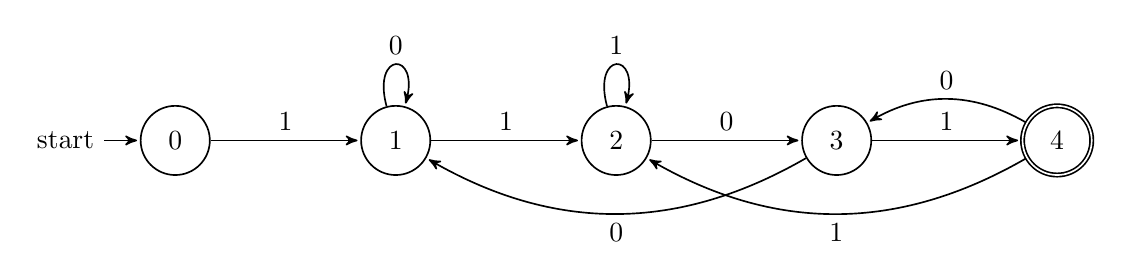
\begin{tikzpicture}[->,>=stealth',shorten >=1pt,auto,node distance=2.8cm, semithick]
            
                \node[initial, state] (0) {0};
                \node[state] (1) [right of=0] {1};
                \node[state] (2) [right of=1] {2};
                \node[state] (3) [right of=2] {3};
                \node[accepting, state] (4) [right of=3] {4};
                
                \path 
                (0) edge node {1} (1)
                (1) edge [loop above] node {0} (1)
                    edge node {1} (2)
                (2) edge node {0} (3)
                    edge [loop above] node {1} (2)
                (3) edge node {1} (4)
                    edge [bend left] node {0} (1)
                (4) edge [bend right] node [above] {0} (3)
                    edge [bend left] node {1} (2)
                ;
            \end{tikzpicture}
            \caption{正规式 1(0|1)*101 的 DFA}
            \label{fig:1_1_5}
        \end{figure}
        
        \item 1(1010*|1(010)*1)*0
        
        首先根据正规式构造 NFA:
        \begin{figure}[H]
            \centering
            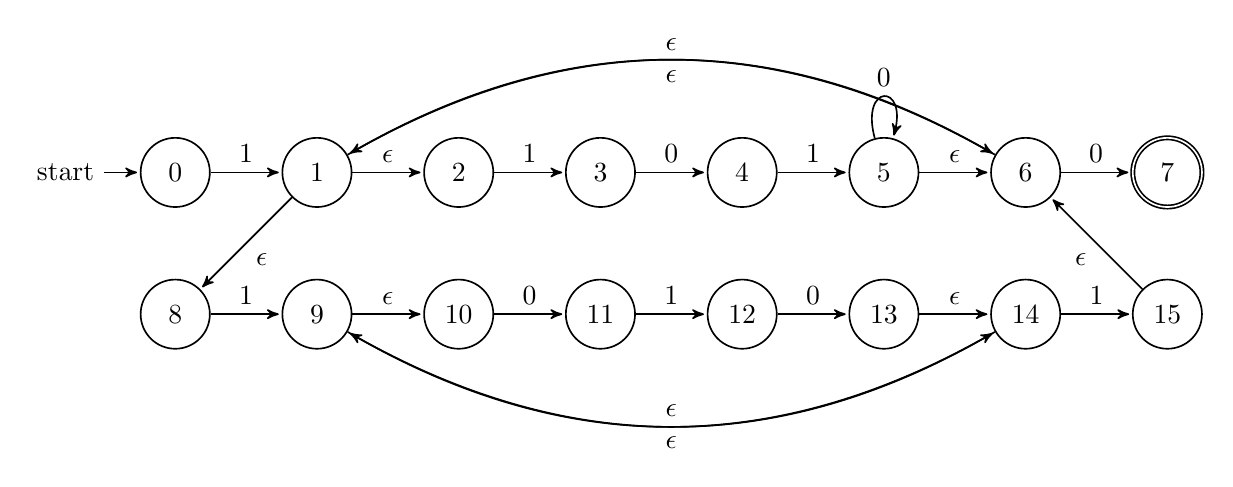
\begin{tikzpicture}[->,>=stealth',shorten >=1pt,auto,node distance=1.8cm,
                                semithick]
                \node[initial, state] (0) {0};
                \node[state] (1) [right of=0] {1};
                \node[state] (2) [right of=1] {2};
                \node[state] (3) [right of=2] {3};
                \node[state] (4) [right of=3] {4};
                \node[state] (5) [right of=4] {5};
                \node[state] (6) [right of=5] {6};
                \node[accepting, state] (7) [right of=6] {7};
                \node[state] (8) [below of=0] {8};
                \node[state] (9) [right of=8] {9};
                \node[state] (10) [right of=9] {10};
                \node[state] (11) [right of=10] {11};
                \node[state] (12) [right of=11] {12};
                \node[state] (13) [right of=12] {13};
                \node[state] (14) [right of=13] {14};
                \node[state] (15) [right of=14] {15};
                
                \path
                (0) edge node {1} (1)
                (1) edge node {$\epsilon$} (2)
                    edge [bend left] node {$\epsilon$} (6)
                    edge node {$\epsilon$} (8)
                (2) edge node {1} (3)
                (3) edge node {0} (4)
                (4) edge node {1} (5)
                (5) edge [loop above] node {0} (5)
                    edge node {$\epsilon$} (6)
                (6) edge [bend right] node {$\epsilon$} (1)
                    edge node {0} (7)
                (8) edge node {1} (9)
                (9) edge node {$\epsilon$} (10)
                    edge [bend right] node {$\epsilon$} (14)
                (10) edge node {0} (11)
                (11) edge node {1} (12)
                (12) edge node {0} (13)
                (13) edge node {$\epsilon$} (14)
                (14) edge [bend left] node {$\epsilon$} (9)
                    edge node {1} (15)
                (15) edge node {$\epsilon$} (6)
                ;
            \end{tikzpicture}
            \caption{正规式 1(1010*|1(010)*1)*0 的直接 NFA}
            \label{fig:1_2_1}
        \end{figure}
        
        重定向边得到 NFA:
        
        并进行了重新标号:$9 \to 2, 11 \to 6, 12 \to 8$
        
        \begin{figure}[H]
            \centering
            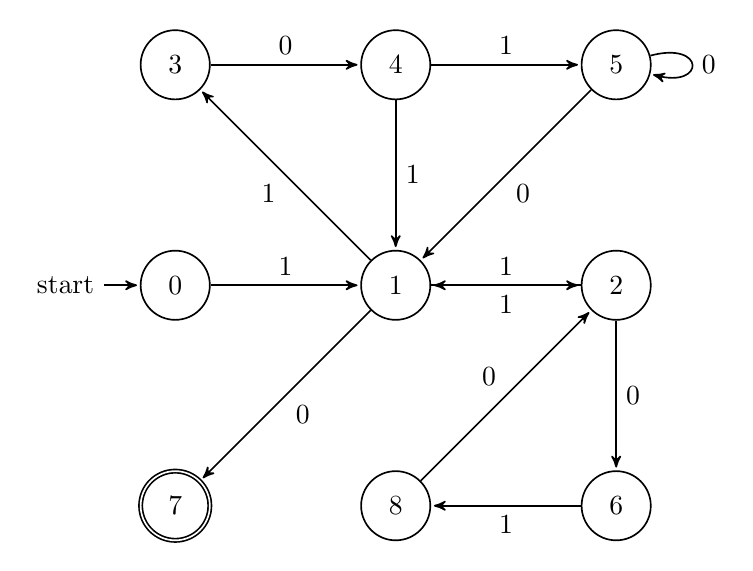
\begin{tikzpicture}[->,>=stealth',shorten >=1pt,auto,node distance=2.8cm,
                                semithick]
                \node[initial, state] (0) {0};
                \node[state] (1) [right of = 0] {1};
                \node[state] (2) [right of = 1] {2};
                \node[state] (3) [above of = 0] {3};
                \node[state] (4) [right of = 3] {4};
                \node[state] (5) [right of = 4] {5};
                \node[state] (6) [below of = 2] {6};
                \node[accepting, state] (7) [below of = 0] {7};
                \node[state] (8) [left of = 6] {8};
                
                \path
                (0) edge node {1} (1)
                (1) edge node {1} (2)
                    edge node {1} (3)
                    edge node {0} (7)
                (2) edge node {1} (1)
                    edge node {0} (6)
                (3) edge node {0} (4)
                (4) edge node {1} (5)
                    edge node {1} (1)
                (5) edge [loop right] node {0} (5)
                    edge node {0} (1)
                (6) edge node {1} (8)
                (8) edge node {0} (2)
                ;
            \end{tikzpicture}
            \caption{正规式 1(1010*|1(010)*1)*0 的化简 NFA}
            \label{fig:1_2_2}
        \end{figure}
        
        计算一步状态转移列表:
        
        \begin{table}[H]
            \centering
            \begin{tabular}{|c|c|c|c|}
                \hline
                n & I & 0 & 1 \\
                \hline
                0 & \{0\} & $\emptyset$ & \{1\} \\
                \hline
                1 & \{1\} & \{7\} & \{2, 3\} \\
                \hline
                2 & \{7\} & $\emptyset$ & $\emptyset$ \\
                \hline
                3 & \{2, 3\} & \{4, 6\} & \{1\} \\
                \hline
                4 & \{4, 6\} & $\emptyset$ & \{1, 5, 8\} \\
                \hline
                5 & \{1, 5, 8\} & \{1, 2, 5, 7\} & \{2, 3\} \\
                \hline
                6 & \{1, 2, 5, 7\} & \{1, 5, 6, 7\} & \{1, 2, 3\} \\
                \hline
                7 & \{1, 5, 6, 7\} & \{1, 5, 7\} & \{2, 3, 8\} \\
                \hline
                8 & \{1, 2, 3\} & \{4, 6, 7\} & \{1, 2, 3\} \\
                \hline
                9 & \{1, 5, 7\} & \{1, 5, 7\} & \{2, 3\} \\
                \hline
                10 & \{2, 3, 8\} & \{2, 4, 6\} & \{1\} \\
                \hline
                11 & \{4, 6, 7\} & $\emptyset$ & \{1, 5, 8\} \\
                \hline
                12 & \{2, 4, 6\} & \{6\} & \{1, 5, 8\} \\
                \hline
                13 & \{6\} & $\emptyset$ & \{8\} \\
                \hline
                14 & \{8\} & \{2\} & $\emptyset$ \\
                \hline
                15 & \{2\} & \{6\} & \{1\} \\
                \hline
            \end{tabular}
            \caption{状态转移表}
            \label{tab:2}
        \end{table}
        
        重新标号得到 DFA。
        
        \begin{figure}[H]
            \centering
            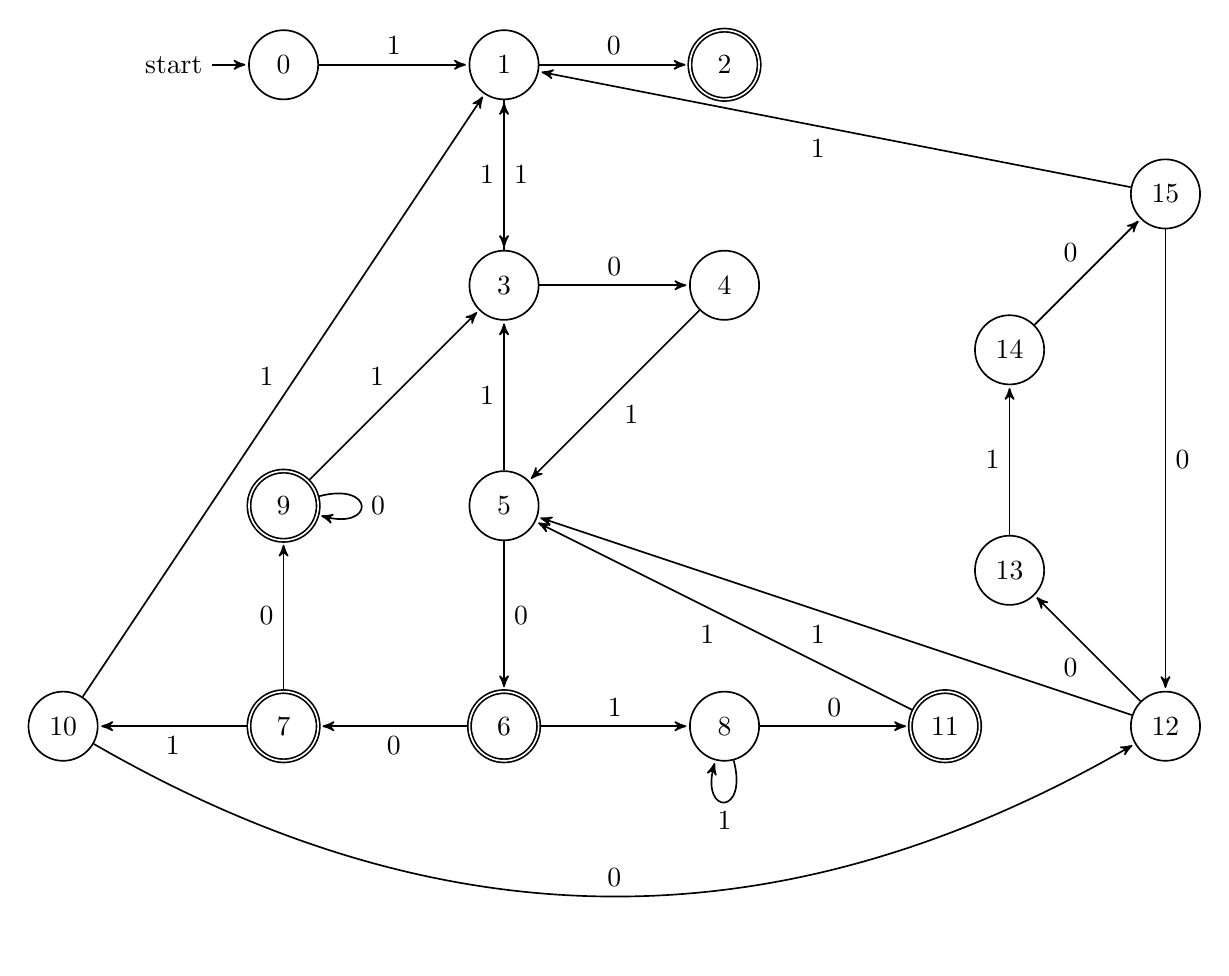
\begin{tikzpicture}[->,>=stealth',shorten >=1pt,auto,node distance=2.8cm,semithick]
                \node[initial, state] (0) {0};
                \node[state] (1) [right of = 0] {1};
                \node[state, accepting] (2) [right of = 1] {2};
                \node[state] (3) [below of = 1] {3};
                \node[state] (4) [right of = 3] {4};
                \node[state] (5) [below of = 3] {5};
                \node[state, accepting] (6) [below of = 5] {6};
                \node[state, accepting] (7) [left of = 6] {7};
                \node[state] (8) [right of = 6] {8};
                \node[state, accepting] (9) [above of = 7] {9};
                \node[state] (10) [left of = 7] {10};
                \node[state, accepting] (11) [right of = 8] {11};
                \node[state] (12) [right of = 11] {12};
                \node[state] (13) [above left of = 12] {13};
                \node[state] (14) [above of = 13] {14};
                \node[state] (15) [above right of = 14] {15};
                
                \path
                (0) edge node {1} (1)
                (1) edge node {0} (2)
                    edge node {1} (3)
                (3) edge node {0} (4)
                    edge node {1} (1)
                (4) edge node {1} (5)
                (5) edge node {0} (6)
                    edge node {1} (3)
                (6) edge node {0} (7)
                    edge node {1} (8)
                (7) edge node {0} (9)
                    edge node {1} (10)
                (8) edge node {0} (11)
                    edge [loop below] node {1} (8)
                (9) edge [loop right] node {0} (9)
                    edge node {1} (3)
                (10) edge [bend right] node {0} (12)
                    edge node {1} (1)
                (11) edge node {1} (5)
                (12) edge node {0} (13)
                    edge node {1} (5)
                (13) edge node {1} (14)
                (14) edge node {0} (15)
                (15) edge node {0} (12)
                    edge node {1} (1)
                ;
            \end{tikzpicture}
            \caption{正规式 1(1010*|1(010)*1)*0 的 DFA}
            \label{fig:1_2_3}
        \end{figure}
        
        \item 0*10*10*10*
        
        这可太简单了直接出结果吧。
        \begin{figure}[H]
            \centering
            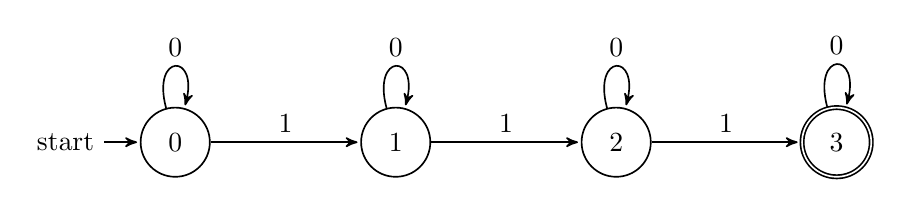
\begin{tikzpicture}[->,>=stealth',shorten >=1pt,auto,node distance=2.8cm,semithick]
                \node[state, initial] (0) {0};
                \node[state] (1) [right of = 0] {1};
                \node[state] (2) [right of = 1] {2};
                \node[state, accepting] (3) [right of = 2] {3};
                \path
                (0) edge [loop above] node {0} (0)
                    edge node {1} (1)
                (1) edge [loop above] node {0} (1)
                    edge node {1} (2)
                (2) edge [loop above] node {0} (2)
                    edge node {1} (3)
                (3) edge [loop above] node {0} (3)
                ;
            \end{tikzpicture}
            \caption{正规式 0*10*10*10* 的 DFA}
            \label{fig:1_3_1}
        \end{figure}
        
        \item (00|11)*((01|10)(00|11)*(01|10)(00|11)*)*
        
        暗中观察发现这个式子中有很多重复的部分。
        
        \begin{figure}[H]
            \begin{subfigure}{0.45\textwidth}
                \centering
                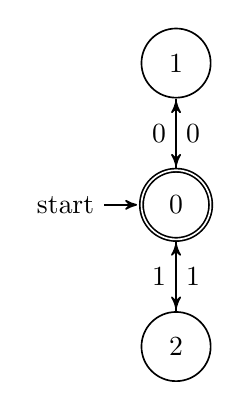
\begin{tikzpicture}[->,>=stealth',shorten >=1pt,auto,node distance=1.8cm,semithick]
                    \node[state, initial, accepting] (0) {0};
                    \node[state] (1) [above of = 0] {1};
                    \node[state] (2) [below of = 0] {2};
                    \path
                    (0) edge node {0} (1)
                        edge node {1} (2)
                    (1) edge node {0} (0)
                    (2) edge node {1} (0)
                    ;
                \end{tikzpicture}
                \caption{(00|11)*}
                \label{fig:subim1}
            \end{subfigure}
            \begin{subfigure}{0.45\textwidth}
                \centering
                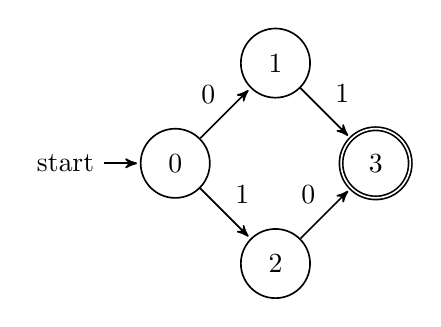
\begin{tikzpicture}[->,>=stealth',shorten >=1pt,auto,node distance=1.8cm,semithick]
                    \node[state, initial] (0) {0};
                    \node[state] (1) [above right of = 0] {1};
                    \node[state] (2) [below right of = 0] {2};
                    \node[state, accepting] (3) [below right of = 1] {3};
                    \path
                    (0) edge node {0} (1)
                        edge node {1} (2)
                    (1) edge node {1} (3)
                    (2) edge node {0} (3)
                    ;
                \end{tikzpicture}
                \caption{(01|10)}
                \label{fig:subim2}
            \end{subfigure}
        \end{figure}
        
        于是重复组合这两个组件,可以得到 NFA:
        
        \begin{figure}[H]
            \centering
            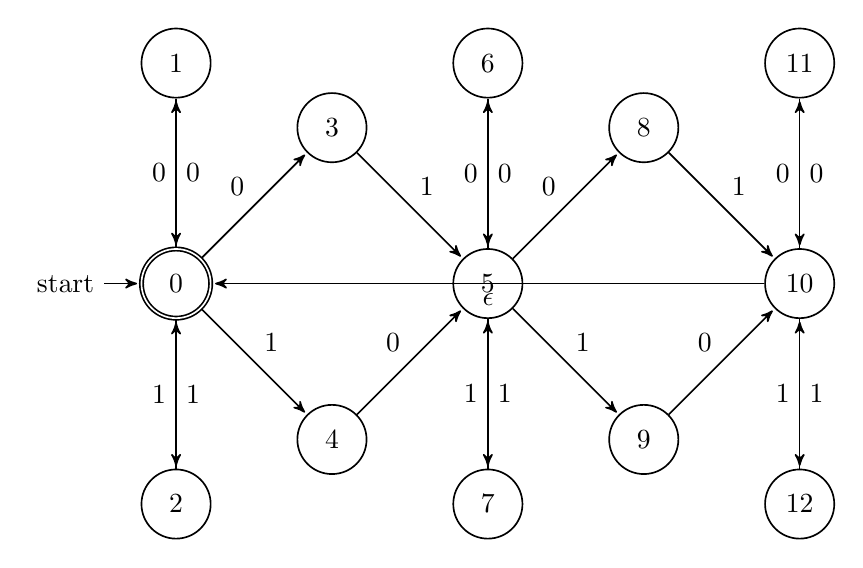
\begin{tikzpicture}[->,>=stealth',shorten >=1pt,auto,node distance=2.8cm,semithick]
                \node[state, initial, accepting] (0) {0};
                \node[state] (1) [above of = 0] {1};
                \node[state] (2) [below of = 0] {2};
                \node[state] (3) [above right of = 0] {3};
                \node[state] (4) [below right of = 0] {4};
                \node[state] (5) [below right of = 3] {5};
                \node[state] (6) [above of = 5] {6};
                \node[state] (7) [below of = 5] {7};
                \node[state] (8) [above right of = 5] {8};
                \node[state] (9) [below right of = 5] {9};
                \node[state] (10) [below right of = 8] {10};
                \node[state] (11) [above of = 10] {11};
                \node[state] (12) [below of = 10] {12};
                
                
                \path
                (0) edge node {0} (1)
                    edge node {1} (2)
                    edge node {0} (3)
                    edge node {1} (4)
                (1) edge node {0} (0)
                (2) edge node {1} (0)
                (3) edge node {1} (5)
                (4) edge node {0} (5)
                (5) edge node {0} (6)
                    edge node {1} (7)
                    edge node {0} (8)
                    edge node {1} (9)
                (6) edge node {0} (5)
                (7) edge node {1} (5)
                (8) edge node {1} (10)
                (9) edge node {0} (10)
                (10) edge node {0} (11)
                    edge node {1} (12)
                    edge node {$\epsilon$} (0) 
                (11) edge node {0} (10)
                (12) edge node {1} (10)
                ;
            \end{tikzpicture}
            \caption{正规式 (00|11)*((01|10)(00|11)*(01|10)(00|11)*)* 的 NFA}
            \label{fig:1_4_1}
        \end{figure}
        
        边重定向后可以消除 0 与 10 之间的 $\epsilon$ 边:
        
        \begin{figure}[H]
            \centering
            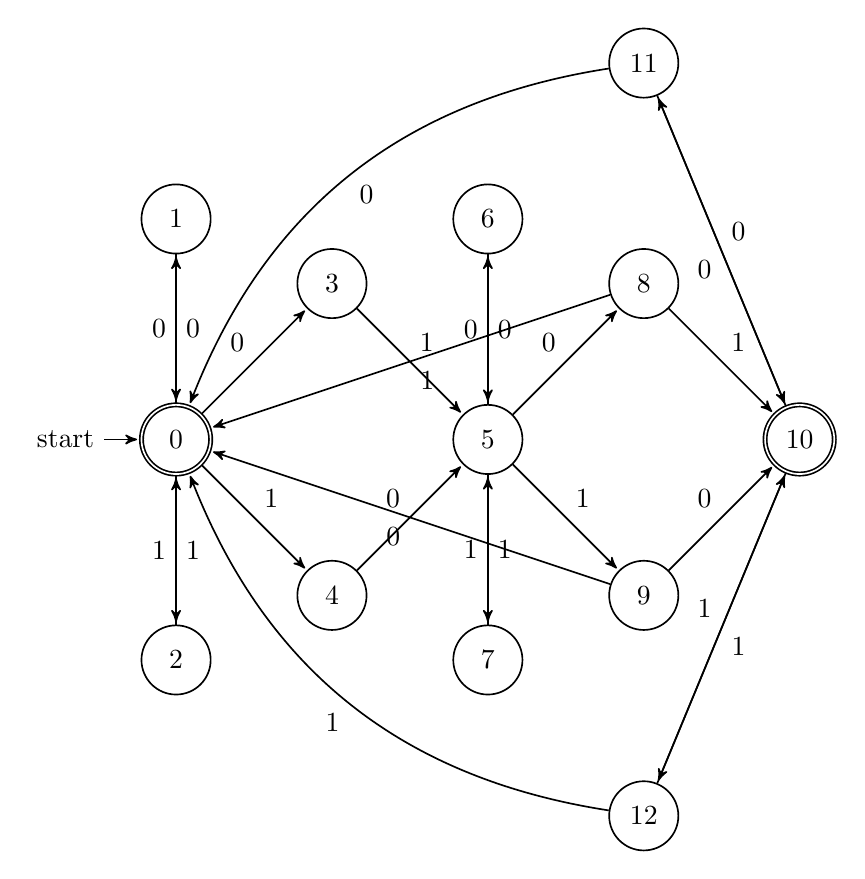
\begin{tikzpicture}[->,>=stealth',shorten >=1pt,auto,node distance=2.8cm,semithick]
                \node[state, initial, accepting] (0) {0};
                \node[state] (1) [above of = 0] {1};
                \node[state] (2) [below of = 0] {2};
                \node[state] (3) [above right of = 0] {3};
                \node[state] (4) [below right of = 0] {4};
                \node[state] (5) [below right of = 3] {5};
                \node[state] (6) [above of = 5] {6};
                \node[state] (7) [below of = 5] {7};
                \node[state] (8) [above right of = 5] {8};
                \node[state] (9) [below right of = 5] {9};
                \node[state, accepting] (10) [below right of = 8] {10};
                \node[state] (11) [above of = 8] {11};
                \node[state] (12) [below of = 9] {12};
                
                
                \path
                (0) edge node {0} (1)
                    edge node {1} (2)
                    edge node {0} (3)
                    edge node {1} (4)
                (1) edge node {0} (0)
                (2) edge node {1} (0)
                (3) edge node {1} (5)
                (4) edge node {0} (5)
                (5) edge node {0} (6)
                    edge node {1} (7)
                    edge node {0} (8)
                    edge node {1} (9)
                (6) edge node {0} (5)
                (7) edge node {1} (5)
                (8) edge node {1} (0)
                    edge node {1} (10)
                (9) edge node {0} (0)
                    edge node {0} (10)
                (10) edge node {0} (11)
                    edge node {1} (12)
                (11) edge node {0} (10)
                    edge [bend right] node {0} (0)
                (12) edge node {1} (10)
                    edge [bend left] node {1} (0)
                ;
            \end{tikzpicture}
            \caption{正规式 (00|11)*((01|10)(00|11)*(01|10)(00|11)*)* 的化简 NFA}
            \label{fig:1_4_2}
        \end{figure}
        
        计算状态转移表:
        
        \begin{table}[H]
            \centering
            \begin{tabular}{|c|c|c|c|}
                \hline
                n & $I$ & $I_0$ & $I_1$ \\
                \hline
                0 & \{0\} & \{1, 3\} & \{2, 4\} \\
                \hline
                1 & \{1, 3\} & \{0\} & \{5\} \\
                \hline
                2 & \{2, 4\} & \{5\} & \{0\} \\
                \hline
                3 & \{5\} & \{6, 8\} & \{7, 9\} \\
                \hline
                4 & \{6, 8\} & \{5\} & \{0, 10\} \\
                \hline
                5 & \{7, 9\} & \{0, 10\} & \{5\} \\
                \hline
                6 & \{0, 10\} & \{1, 3, 11\} & \{2, 4, 12\} \\
                \hline
                7 & \{1, 3, 11\} & \{0\} & \{5\} \\
                \hline
                8 & \{2, 4, 12\} & \{5\} & \{0\} \\
                \hline
            \end{tabular}
            \caption{状态转移表}
            \label{tab:4}
        \end{table}
        
        暗中观察发现表 \ref{tab:4} 中 n 的值属于 {1, 7} 的 $I_0, I_1$ 对应相同,{2, 8}, {0, 6} 也具有同样的性质,这表明 {0, 6}, {1, 7}, {2, 8} 可以分别合并为 0, 1, 2。
        
        \begin{table}[H]
            \centering
            \begin{tabular}{|c|c|c|c|}
                \hline
                n & $I$ & $I_0$ & $I_1$ \\
                \hline
                0 & \{0\} & 1 & 2 \\
                \hline
                1 & \{1, 3\} & 0 & 3 \\
                \hline
                2 & \{2, 4\} & 3 & 0 \\
                \hline
                3 & \{5\} & 4 & 5 \\
                \hline
                4 & \{6, 8\} & 3 & 0 \\
                \hline
                5 & \{7, 9\} & 0 & 3 \\
                \hline
            \end{tabular}
            \caption{简化的状态转移表}
            \label{tab:4_1}
        \end{table}
        
        随后继续观察发现 {1, 5}, {2, 4} 也出现了这样的性质,继续合并到 1, 2。
        
        \begin{table}[H]
            \centering
            \begin{tabular}{|c|c|c|c|}
                \hline
                n & $I$ & $I_0$ & $I_1$ \\
                \hline
                0 & \{0\} & 1 & 2 \\
                \hline
                1 & \{1, 3\} & 0 & 3 \\
                \hline
                2 & \{2, 4\} & 3 & 0 \\
                \hline
                3 & \{5\} & 2 & 1 \\
                \hline
            \end{tabular}
            \caption{最简化的状态转移表}
            \label{tab:4_3}
        \end{table}
        
        
        可视化表 \ref{tab:4_3} 得到 DFA:
        \begin{figure}[H]
            \centering
            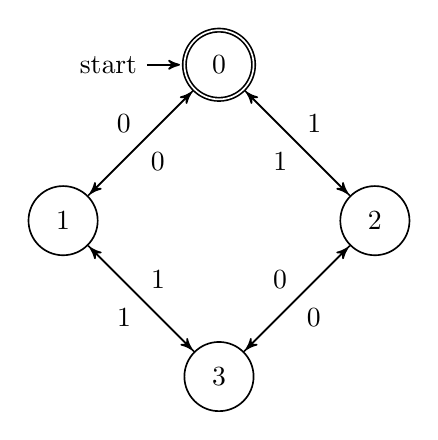
\begin{tikzpicture}[->,>=stealth',shorten >=1pt,auto,node distance=2.8cm,semithick]
                \node[state, initial, accepting] (0) {0};
                \node[state] (1) [below left of = 0] {1};
                \node[state] (2) [below right of = 0] {2};
                \node[state] (3) [below right of = 1] {3};
                \path
                (0) edge node {0} (1)
                    edge node {1} (2)
                (1) edge node {1} (3)
                    edge node {0} (0)
                (2) edge node {0} (3)
                    edge node {1} (0)
                (3) edge node {0} (2)
                    edge node {1} (1)
                ;
                
            \end{tikzpicture}
            \caption{正规式 (00|11)*((01|10)(00|11)*(01|10)(00|11)*)* 的 DFA}
            \label{fig:1_4_3}
        \end{figure}
        

        
    \end{itemize}

	\item[3.9] 对下面情况给出DFA及正规表达式:
	\begin{enumerate}
		\item \{0,1\}上的含有子串 010 的所有串;
		
		\textbf{答:}
		
		构造正规式:(0|1)*010(0|1)*
		
		\begin{figure}[H]
		    \centering
            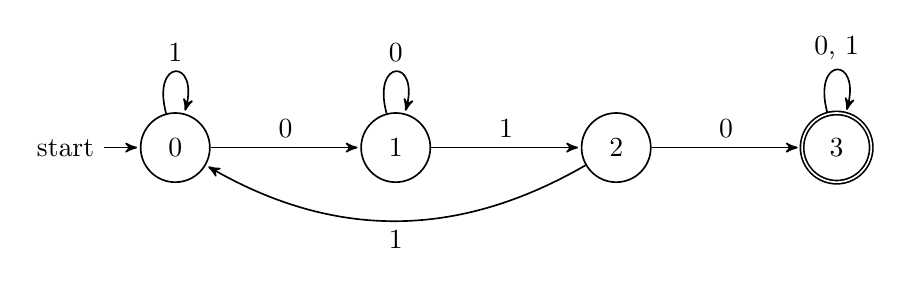
\begin{tikzpicture}[->,>=stealth',shorten >=1pt,auto,node distance=2.8cm,semithick]
		        
		        \node[state, initial] (0) {0};
		        \node[state] (1) [right of = 0] {1};
		        \node[state] (2) [right of = 1] {2};
		        \node[state, accepting] (3) [right of = 2] {3};
		        
		        \path
		        (0) edge node {0} (1)
		            edge [loop above] node {1} (0)
		        (1) edge [loop above] node {0} (1)
		            edge node {1} (2)
		        (2) edge node {0} (3)
		            edge [bend left] node {1} (0)
		        (3) edge [loop above] node {0, 1} (3)
		        ;
		    \end{tikzpicture}
		    \caption{(0|1)*010(0|1)* 对应的 DFA}
		    \label{fig:2_1}
		\end{figure}
		
		\item \{0,1\}上不含字串 010 的所有串。
		
		\textbf{答:}
		
		构造正规式:1*(0*11+)*0*(01)?
		
		\begin{figure}[H]
		    \centering
            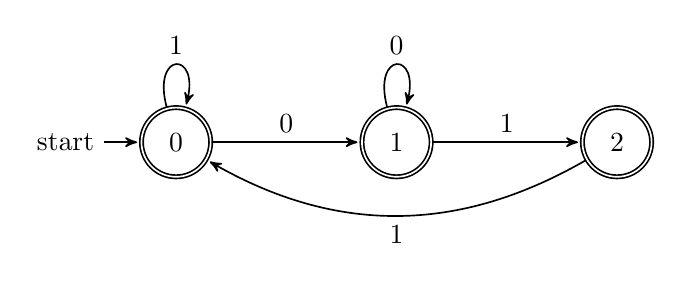
\begin{tikzpicture}[->,>=stealth',shorten >=1pt,auto,node distance=2.8cm,semithick]
		        
		        \node[state, initial, accepting] (0) {0};
		        \node[state, accepting] (1) [right of = 0] {1};
		        \node[state, accepting] (2) [right of = 1] {2};
		        
		        \path
		        (0) edge node {0} (1)
		            edge [loop above] node {1} (0)
		        (1) edge [loop above] node {0} (1)
		            edge node {1} (2)
		        (2) edge [bend left] node {1} (0)
		        ;
		    \end{tikzpicture}
		    \caption{1*(0*11+)*0*(01)? 对应的 DFA}
		    \label{fig:2_2}
		\end{figure}
		
	\end{enumerate}

	\item[3.12] 将图 \ref{fig:3} 的 (\ref{fig:3_1}) 和 (\ref{fig:3_2}) 分别确定化和最少化。
	
    \begin{figure}[H]
        \begin{subfigure}{0.45\textwidth}
            \centering
            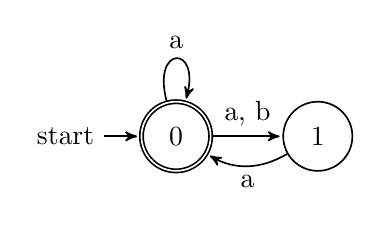
\begin{tikzpicture}[->,>=stealth',shorten >=1pt,auto,node distance=1.8cm,semithick]
                \node[state, initial, accepting] (0) {0};
                \node[state] (1) [right of = 0] {1};
                \path
                (0) edge [loop above] node {a} (0)
                    edge node {a, b} (1)
                (1) edge [bend left] node {a} (0)
                ;
            \end{tikzpicture}
            \caption{}
            \label{fig:3_1}
        \end{subfigure}
        \begin{subfigure}{0.45\textwidth}
            \centering
            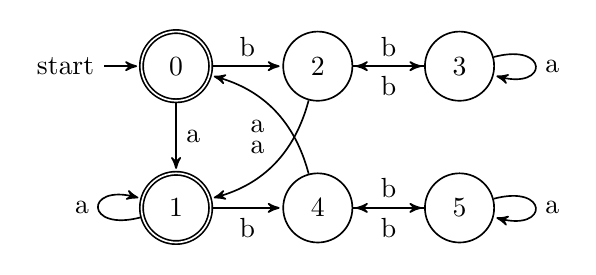
\begin{tikzpicture}[->,>=stealth',shorten >=1pt,auto,node distance=1.8cm,semithick]
                \node[state, initial, accepting] (0) {0};
                \node[state, accepting] (1) [below of = 0] {1};
                \node[state] (2) [right of = 0] {2};
                \node[state] (3) [right of = 2] {3};
                \node[state] (4) [right of = 1] {4};
                \node[state] (5) [right of = 4] {5};
                \path
                (0) edge node {a} (1)
                    edge node {b} (2)
                (1) edge [loop left] node {a} (1)
                    edge node [below] {b}(4)
                (2) edge [bend left] node [above left] {a} (1)
                    edge node {b} (3)
                (3) edge [loop right] node {a} (3)
                    edge node {b} (2)
                (4) edge [bend right] node {a} (0)
                    edge node {b} (5)
                (5) edge [loop right] node {a} (5)
                    edge node {b} (4)
                ;
            \end{tikzpicture}
            \caption{}
            \label{fig:3_2}
        \end{subfigure}
        \caption{}
        \label{fig:3}
    \end{figure}
    
    \textbf{答:}
    
    确定化:
    
    图 \ref{fig:3_1} 并不是 DFA 所以要做确定化,而图 \ref{fig:3_2} 所示是 DFA 不需要确定化。
    
    \begin{figure}[H]
        \begin{subfigure}{0.45\textwidth}
            \centering
            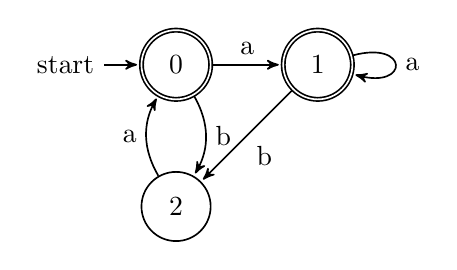
\begin{tikzpicture}[->,>=stealth',shorten >=1pt,auto,node distance=1.8cm,semithick]
                \node[state, initial, accepting] (0) {0};
                \node[state, accepting] (1) [right of = 0] {1};
                \node[state] (2) [below of = 0] {2};
                \path
                (0) edge node {a} (1)
                    edge [bend left] node {b} (2)
                (1) edge [loop right] node {a} (1)
                    edge node {b} (2)
                (2) edge [bend left] node {a} (0)
                ;
            \end{tikzpicture}
            \caption{}
            \label{fig:3_ans_1_a}
        \end{subfigure}
        \begin{subfigure}{0.45\textwidth}
            \centering
            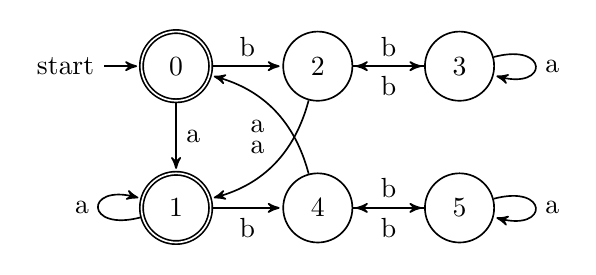
\begin{tikzpicture}[->,>=stealth',shorten >=1pt,auto,node distance=1.8cm,semithick]
                \node[state, initial, accepting] (0) {0};
                \node[state, accepting] (1) [below of = 0] {1};
                \node[state] (2) [right of = 0] {2};
                \node[state] (3) [right of = 2] {3};
                \node[state] (4) [right of = 1] {4};
                \node[state] (5) [right of = 4] {5};
                \path
                (0) edge node {a} (1)
                    edge node {b} (2)
                (1) edge [loop left] node {a} (1)
                    edge node [below] {b}(4)
                (2) edge [bend left] node [above left] {a} (1)
                    edge node {b} (3)
                (3) edge [loop right] node {a} (3)
                    edge node {b} (2)
                (4) edge [bend right] node {a} (0)
                    edge node {b} (5)
                (5) edge [loop right] node {a} (5)
                    edge node {b} (4)
                ;
            \end{tikzpicture}
            \caption{}
            \label{fig:3_ans_1_b}
        \end{subfigure}
        \caption{}
        \label{fig:3_ans_1}
    \end{figure}
    
    最小化:
    
    暗中观察发现如下结论:
    
    \begin{itemize}
        \item 图 \ref{fig:3_ans_1_a} 中 \{0, 1\} 不能被任何串区分,并且 \{0, 1\}, \{2\} 可以被区分。
        
        \item 图 \ref{fig:3_ans_1_b} 中 \{0, 1\}, \{2, 4\}, \{3, 5\} 可以分别合并。
    \end{itemize}
    
    所以得到最小化 DFA:
    
    \begin{figure}[H]
        \begin{subfigure}{0.45\textwidth}
            \centering
            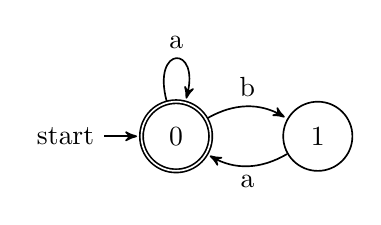
\begin{tikzpicture}[->,>=stealth',shorten >=1pt,auto,node distance=1.8cm,semithick]
                \node[state, initial, accepting] (0) {0};
                \node[state] (1) [right of = 0] {1};
                \path
                (0) edge [loop above] node {a} (0)
                    edge [bend left] node {b} (1)
                (1) edge [bend left] node {a} (0)
                ;
            \end{tikzpicture}
            \caption{}
            \label{fig:3_ans_2_a}
        \end{subfigure}
        \begin{subfigure}{0.45\textwidth}
            \centering
            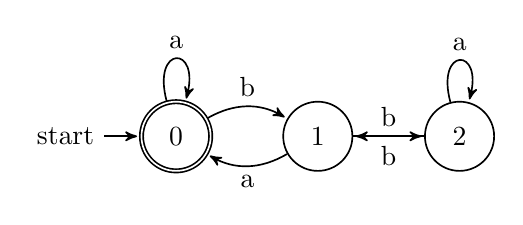
\begin{tikzpicture}[->,>=stealth',shorten >=1pt,auto,node distance=1.8cm,semithick]
                \node[state, initial, accepting] (0) {0};
                \node[state] (1) [right of = 0] {1};
                \node[state] (2) [right of = 1] {2};
                \path
                (0) edge [loop above] node {a} (0)
                    edge [bend left] node {b} (1)
                (1) edge [bend left] node {a} (0)
                    edge node {b} (2)
                (2) edge [loop above] node {a} (2)
                    edge node {b} (1)
                ;
            \end{tikzpicture}
            \caption{}
            \label{fig:3_ans_2_b}
        \end{subfigure}
        \caption{}
        \label{fig:3_ans_2}
    \end{figure}
    
    
    \item[3.14] 构造一个DFA,它接收$\Sigma=\{0,1\}$上所有满足如下条件的字符串:每个1都有0直接跟在右边。
	
	\textbf{答:}
	
	构造正规式 0*(10+)*,转换成 DFA:
	
	\begin{figure}[H]
        \centering
        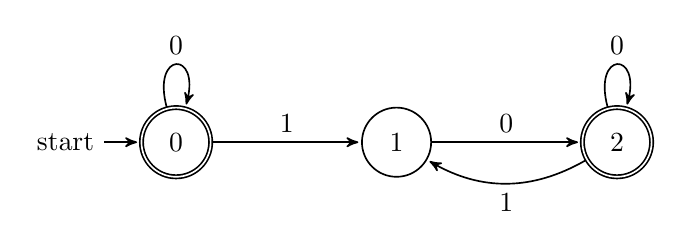
\begin{tikzpicture}[->,>=stealth',shorten >=1pt,auto,node distance=2.8cm,semithick]
            
            \node[state, initial, accepting] (0) {0};
            \node[state] (1) [right of = 0] {1};
            \node[state, accepting] (2) [right of = 1] {2};
            
            \path
            (0) edge node {1} (1)
                edge [loop above] node {0} (0)
            (1) edge node {0} (2)
            (2) edge [bend left] node {1} (1)
                edge [loop above] node {0} (2)
            ;
        \end{tikzpicture}
        \caption{0*(10+)* 对应的 DFA}
        \label{fig:4}
    \end{figure}
    
    合并 \{0, 2\} 
    
	\begin{figure}[H]
        \centering
        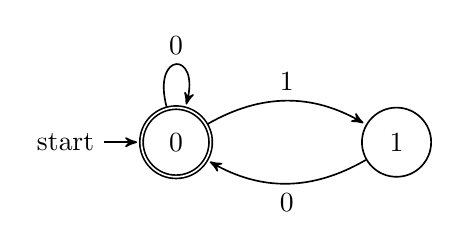
\begin{tikzpicture}[->,>=stealth',shorten >=1pt,auto,node distance=2.8cm,semithick]
            
            \node[state, initial, accepting] (0) {0};
            \node[state] (1) [right of = 0] {1};
            
            \path
            (0) edge [bend left] node {1} (1)
                edge [loop above] node {0} (0)
            (1) edge [bend left] node {0} (0)
            ;
        \end{tikzpicture}
        \caption{0*(10+)* 对应的最简 DFA}
        \label{fig:4_1}
    \end{figure}
    
	
\end{enumerate}

\end{document}
